\section{Concept}
\label{section:concept}
In this section a concept of a mobile \gls{see} version will be presented. 
Therefore, a prototype will be created to point out the features that a mobile version of \gls{see} requires.

Prototypes are a common way to express the needs of a system. 
It is a low-cost way of planning an implementation, that can highlight challenges regarding constraints of a system early on.

Even though a prototype will never be able to show every aspect and need of a complex system, it should still help to answering questions like: 
How should the system feel? How should it be implemented, and what are the key features? \cite{houde1997prototypes} 

\gls{see} is meant to be used by multiple platforms such as desktop devices, mobile devices and virtual reality devices.
Each device has different interaction constrains. 
While a desktop user will control the player with mouse and keyboard a mobile user will interact with virtual joysticks on a touchscreen.
Selecting nodes of a \gls{city} will be done by clicking it with a mouse on desktop devices, while a mobile device will require a touch input.

\subsection{Interface}

In the following a paper prototype will be presented that marks out a concept for the mobile interface.
Since the field of mobile development is quite young there few guidelines regarding the design of mobile device interfaces.
A guideline that is widely accepted is problematic to find. \cite{renaud2017demarcating}, \cite{punchoojit2017usability}

Major differences to desktop environments are the screen size, forms of input and input feedback.
To assure as much space is used for the actual interaction of the app the menu should just take as much space as needed.
As a study has found out, a size of at least 8*8 mm is needed to reduce error rates selecting the right button. \cite{conradi2015optimal} \cite{parhi2006target}
TODO WEITER AUSFÜHREN
SHORTCUTS WIE STRG Z NICHT MÖGLICH
 \cite{adipat2005interface} 

Moving the player will be handled with virtual joysticks as seen in figure \ref{fig:joystick}.
The left joystick will move the player through the virtual room and the right will move the camera angle or in other word the direction the player looks at.
The joysticks are placed in the left and right corner and should just take as much space as needed to be handled comfortably.
This way the player is able to navigate through the virtual room with his/her thumps while still having enough space to work on the \gls{city}.

\begin{figure}[htb]
    \centering
    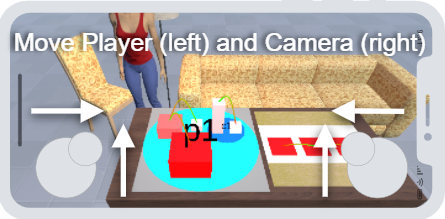
\includegraphics[width=1\textwidth]{Concept/img/joystick.png}
    \caption{Joysticks for moving in \gls{see}}\label{fig:joystick}
\end{figure}

The menu on the top left side seen in figure \ref{fig:quickbar} will be called "quickbar" further on. 
The quickbar can be minimized to safe screen space when not needed. 
The quickbar is designed to offer more general functions that are needed in various situations.
Because there are no shortcuts on mobile devices each function has to have a button to be activated.

The functions are redo and undo which will do an action undone again or revert an action.
Then there is a camera lock that will lock the players perspective to a certain \gls{city} so that the player can only move around the selected city and move closer or further away from it.
The next function is to rerotate a \gls{city}.
That means the \gls{city} that was last rotated will be set back to its initial state of rotation.
Last but not least there will be a button for recentering the city, which will work quite similar to the rerotate button and center the last moved \gls{city}.
The button on the right can be used to collapse or expand the quickbar.
\begin{figure}[htb]
    \centering
    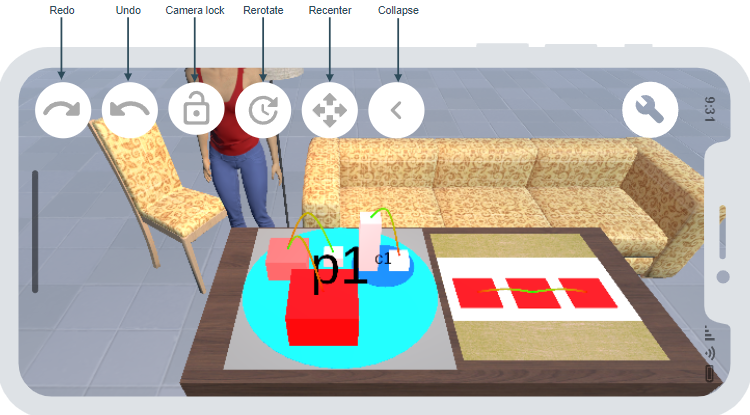
\includegraphics[width=1\textwidth]{Concept/img/quickbar.png}
    \caption{Quickbar for various interactions in \gls{see}}\label{fig:quickbar}
\end{figure}

On the top right side another menu will be placed that contains different interaction modes.
By clicking a button an interaction mode will be selected and moved to the top right corner.
Also, the menu will be collapsed and only the buttons regarding the selected interaction mode shall be shown.
By clicking the button on the top right again the menu shall expand and the other interaction modes shall be selectable.
The other buttons shall be kept in the same order to reduce confusion of the user.

The first interaction mode, seen in figure \ref{fig:select}, is for selecting nodes.
Nodes can be selected by being touched and deselected by being touched again.
There can be multiple nodes selected at once.
The hole selection can be deselected by clicking the deselect button next to the select interaction mode button.
Selected nodes shall be highlighted with a different node color and also display their name.

\begin{figure}[htb]
    \centering
    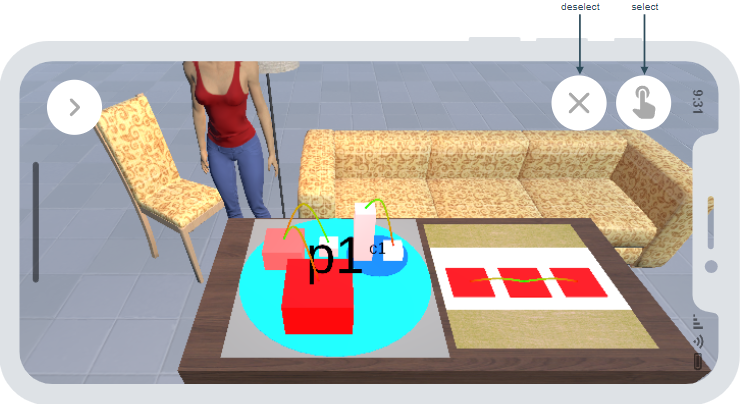
\includegraphics[width=1\textwidth]{Concept/img/menu1.png}
    \caption{Selection mode in \gls{see}}\label{fig:select}
\end{figure}

The second interaction mode, seen in figure \ref{fig:delete}, is for deleting node.
It does not need additional buttons.
Node will be deleted by being touched.-
Unlike in the desktop version there will not be a group deletion interaction because it would require an additional menu panel.
The added functionality would be minimal and selecting a group of nodes, confirming and finally deleting would require a handful more steps and would therefore most likely not be used.

\begin{figure}[htb]
    \centering
    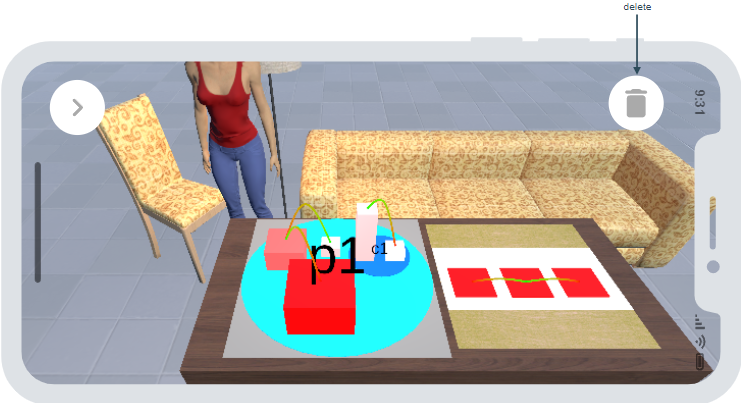
\includegraphics[width=1\textwidth]{Concept/img/menu2.png}
    \caption{Delete mode in \gls{see}}\label{fig:delete}
\end{figure}

The following interaction mode, seen in figure \ref{fig:nodes}, is dedicated to the nodes and edges of a \gls{city}.
Starting on with the "add node" button on the right.
When activated the user can create new node by clicking on a certain spot on the \gls{city} plane. 
The following button on the left is for adding edges.
By selecting two nodes a new edge will be created between them. 
Then, the button one further on the right is for editing nodes.
By touching a node a window will pop up that allows the user to edit the node by changing its name and its type.
Last but not least the button on the left-hand side will be used to scale nodes.
That means the node height and width can be adjusted by first selecting it via touch and then hold a corner and slide it further away from the node center to increase the size or slide it towards the center to decrease the size of the node.
Each button of the node interactions will be marked green after being pressed to indicate that it is active.

\begin{figure}[htb]
    \centering
    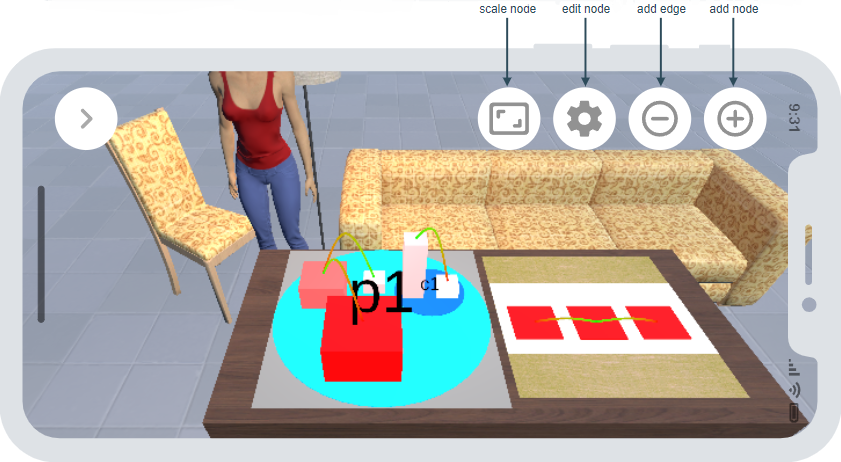
\includegraphics[width=1\textwidth]{Concept/img/menu3.png}
    \caption{Node interactions in \gls{see}}\label{fig:nodes}
\end{figure}

Then there will be a button for rotation interactions that can be seen in figure \ref{fig:rotate}.
Starting with the first activatable button that lets the user rotate the hole \gls{city} by touching any point on it and then sliding away from that point.
Similar to that there will be a button that lets the user rotate just a single node on the \gls{city}.
In addition to that there will be a button that activates the so-called "locked-rotation" mode.
While in "locked-rotation" mode the rotation of a node or \gls{city} will be done in eight predefined steps to a full rotation.
Each step will have the same 45° range.
The last button of this group will be for changing the center of the rotations. 
There are to options: the first option is a center of rotation in the middle of the \gls{city} and the second is in the middle of a node selection made with the interactions seen in figure \ref{fig:select}.
The second option can be activated by pressing the last button.

\begin{figure}[htb]
    \centering
    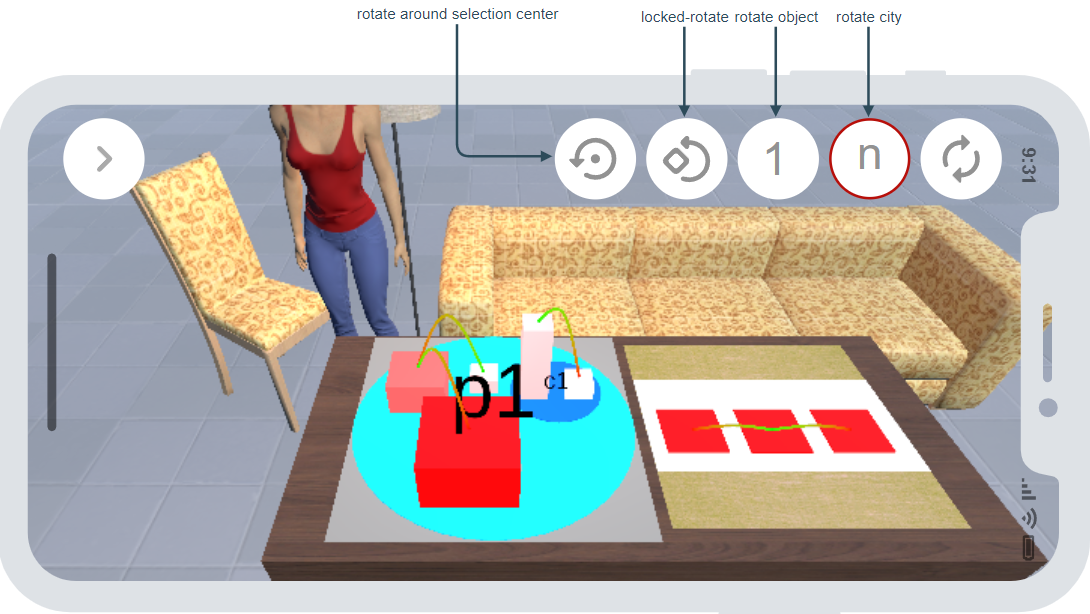
\includegraphics[width=1\textwidth]{Concept/img/menu4.png}
    \caption{Rotation mode in \gls{see}}\label{fig:rotate}
\end{figure}

The last interaction group, seen in figure \ref{fig:move}, is for moving the \gls{city} or a single node.
The move interactions are quite similar to the rotation interactions.
There will be a button to move a hole \gls{city} as well as a button to move only single nodes.
In addition to that there will be a button that restricts the movement of the \gls{city} or node to a predefined direction.
The directions will be again in 45° angles and objects can be moved on a straight line on that angle.
Moving a node or a \gls{city} can be achieved by touching and holding it and then moving it to the desired position.
\begin{figure}[htb]
    \centering
    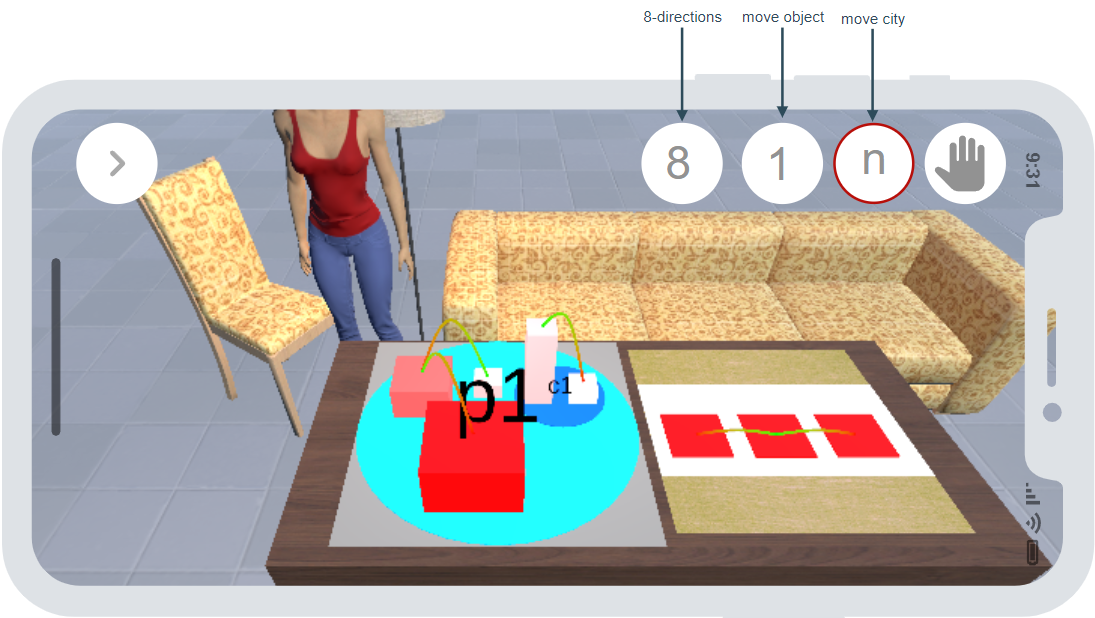
\includegraphics[width=1\textwidth]{Concept/img/menu5.png}
    \caption{Movement mode in \gls{see}}\label{fig:move}
\end{figure}

\subsection{Interaction}

Smartphones are quite limited in space and there are few input possibilities.
Unlike a desktop computer there is no mouse and there is no physical keyboard.
Smartphones use virtual keyboards but due to the restriction of screen space the keyboard is hidden most of the time.
Which would make keyboard shortcuts uncomfortable because the user has to open the keyboard first.
Therefore, smartphones need different ways of interaction such as touch gestures. 

Zooming in to a \gls{city} happens by scrolling on a desktop environment. 
The is no option to scroll on mobile devices, but there are at least two popular alternatives.
The first option would be to double tap on the \gls{city} to zoom in.
The double tap would zoom in, in predefined steps and after reaching a certain level of closeness it would trigger to zoom out again.
In \gls{see} zooming in, in predefined steps might not be precise enough because there could be a quite large \gls{city} or a rather small one.
Finding predefined steps that would fit every situation is rather hard.
Therefore, a second option by zooming in with a two finger gesture might be better. 
In this option the user uses two fingers and slides them towards each other to zoom in or slides the two fingers away from each other to zoom out.
This way there are no predefined steps necessary and zooming interactions can be done precisely.
\subsection{Requirements}
In the following a list of requirements will be given, which will specify in detail what the implementation of a mobile version has to take care of.
The list will be referred to multiple times in the upcoming realization part in chapter \ref{section:implementation}.
Requirements are essential for the planning phase as they give a good fundamental structure for the developer to rely on. \cite{Robertson2012,Stevens2005}
\begin{itemize}
    \item[{[R1]}] The application shall run on Android devices
    \item[{[R2]}] The application shall be controlled via touchscreen
    \begin{itemize}
        \item [{[R2.1]}] The player and camera shall be moved with virtual joysticks
        \item [{[R2.2]}] Needed shortcuts of the desktop version shall be handled with buttons
        \item [{[R2.3]}] Zooming shall be handled with a two finger gesture
    \end{itemize}
    \item[{[R3]}] The user shall be able to select a node of a \gls{city}
    \begin{itemize}
        \item [{[R3.1]}] After selecting the name of the node shall be shown
        \item [{[R3.2]}] The user shall be able to deselect single nodes or a group of nodes
    \end{itemize}
    \item[{[R4]}] The user shall be able to delete nodes
    \item[{[R5]}] The user shall be able to interact with nodes
    \begin{itemize}
        \item [{[R5.1]}] The user shall be able to add nodes
        \item [{[R5.2]}] The user shall be able to add edges
        \item [{[R5.3]}] The user shall be able to edit nodes
        \item [{[R5.4]}] The user shall be able to scale nodes
    \end{itemize}
    \item[{[R6]}] The user shall be able to rotate a \gls{city}
    \begin{itemize}
        \item[{[R6.1]}] The user shall be able to rotate a \gls{city} in 45° steps
        \item[{[R6.2]}] The user shall be able to rotate single objects
        \item[{[R6.3]}] The user shall be able to rotate around a center of selected nodes
        \item[{[R6.4]}] The user shall be able to undo the rotation
    \end{itemize}
    \item[{[R7]}] The user shall be able to move a \gls{city}
    \begin{itemize}
        \item[{[R7.1]}] The user shall be able to move single object of a \gls{city}
        \item[{[R7.2]}] The user shall be able to restore the \gls{city} initial position
        \item[{[R7.3]}] The user shall be able to move a \gls{city} or single node in predefined directions
    \end{itemize}
    \item[{[R8]}] The user shall be able to undo and redo actions
    \item[{[R9]}] The user shall be able to lock the camera to a selected \gls{city}
\end{itemize}